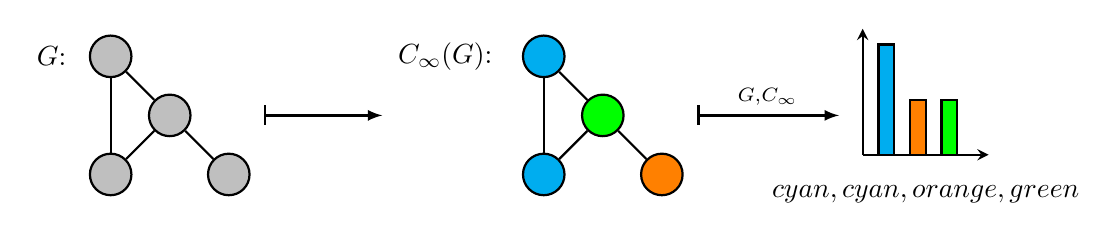
\begin{tikzpicture}
    \tikzset{line/.style={draw,thick}}
    \tikzset{arrow/.style={line,->,>=stealth}}
    \tikzset{node/.style={circle,inner sep=0pt,minimum width=15pt}}
    
    \draw (-1.5 - 1.5,0.75) node {$G$:};
    \node[line,node,fill=lightgray] (x1) at (-0.75 - 1.5, 0.75) {};
    \node[line,node,fill=lightgray] (x2) at (-0.75 - 1.5, -0.75) {};
    \node[line,node,fill=lightgray] (x3) at (0.75 - 1.5, -0.75) {};
    \node[line,node,fill=lightgray] (x4) at (0 - 1.5, 0) {};
    
    \path[line] (x1) to (x2);
    \path[line] (x1) to (x4);
    \path[line] (x2) to (x4);
    \path[line] (x3) to (x4);

    \draw [|-latex, thick] (1.2 - 1.5,0) -- node [text width=2.5cm,midway,above,align=center ] {$\wl$} (2.7 - 1.5,0);
    
    \draw (3.25 - 1.25, 0.75) node {$C_\infty(G)$:};

    \node[line,node,fill=cyan] (x1) at (-0.75 + 4.0, 0.75) {};
    \node[line,node,fill=cyan] (x2) at (-0.75 + 4.0, -0.75) {};
    \node[line,node,fill=orange] (x3) at (0.75 + 4.0, -0.75) {};
    \node[line,node,fill=green] (x4) at (0 + 4.0, 0) {};
    
    \path[line] (x1) to (x2);
    \path[line] (x1) to (x4);
    \path[line] (x2) to (x4);
    \path[line] (x3) to (x4);

    \draw [|-latex, thick] (5.2,0) -- node [text width=2.5cm,midway,above,align=center ] {$\hist_{G, C_\infty}$} (6.7 + 0.3, 0);
    
    \filldraw[draw=black, fill=cyan, thick] (6.2 + 1.0+ 0.3, -0.5) rectangle (6.4 + 1.0+ 0.3, 0.9);
    \filldraw[draw=black, fill=orange, thick] (6.6 + 1.0+ 0.3, -0.5) rectangle (6.8 + 1.0+ 0.3, 0.2);
    \filldraw[draw=black, fill=green, thick] (7.0 + 1.0+ 0.3, -0.5) rectangle (7.2 + 1.0+ 0.3, 0.2);

    \draw[arrow, thick] (6.0 + 1.0+ 0.3, -0.5) to (7.6 + 1.0+ 0.3, -0.5);
    \draw[arrow, thick] (6.0 + 1.0+ 0.3, -0.5) to (6.0 + 1.0+ 0.3, 1.1);

    \draw (7.8+ 0.3, -1.0) node {$\MSopen \sqbox{cyan}, \sqbox{cyan}, \sqbox{orange}, \sqbox{green} \MSclose$};


    \end{tikzpicture}
